%======================================================================
\chapter{Example \LaTeX\ Commands for Typical Large Documents}
\markright{Example \LaTeX\ Commands for Typical Large Documents}
%======================================================================
For details of the many \LaTeX\ commands, the reference books are indispensable.
However, examples of some structures you will likely need are given here.

\LaTeX\ formatting tags include both \emph{commands} and \emph{environments}.
A command is like a switch; it turns a certain mode on until it is changed or ended by the extent of its ``scope'', delimited by curly braces (or by default, such as the end of a paragraph).
Examples of commands are ``\verb=\emph{really} big='' to emphasize a word and ``\verb=\large='' to turn on large text until it is changed again.
An environment has an explicitly defined scope, indicated by \cmmd{begin} and \cmmd{end} commands, \eg \verb=\begin{equation} ... \end{equation}=.
All commands also have an environment form.
See the Glossary of Terms on page~\pageref{chap.glossary} for more key concepts. 
%======================================================================
\section{Selected Text Structures}
%======================================================================
\subsection{Basic In-Line Commands}
%----------------------------------------------------------------------
\begin{itemize}
\item \LaTeX\ ignores    extra   spaces    in the input.
Add space with \verb*=\ =, \ie\ $\backslash$ followed by a space.
\item Separate paragraphs with a blank line.
\item \LaTeX\ ignores anything after a \% character (comment symbol).
\item \emph{Emphasize} text with the \cmmd{emph} command (italicizes).
\item \LaTeX\ recognizes three types of dashes
	\begin{itemize}
	\item Punctuation ( - - - , or \cmmd{textmdash}): He jumped --- but not high enough!
	\item Range ( - - , or \cmmd{textndash}): Read chapters 1--12 for tomorrow's class.
	\item Interword ( - ): What a thought-provoking essay!
	\end{itemize}
\item Use pairs of opening and closing \emph{single} quotes rather than double quotes, to get ``this'' rather than "this".
\item Ellipsis \ldots\ is produced with the \cmmd{ldots} command.
\item Produce some of \LaTeX 's special symbols with a backslash preceding them \eg\ produce \$, \&, \%, \#, \_, \{ and  \} with \cmmd{\$}, \etc .
\item Produce the remaining special characters \verb=\=, \verb=~=, and \verb=^=, with the \cmmd{verb} command or inside a \enviro{verbatim} environment, or use text mode commands: \cmmd{textbackslash}, \cmmd{textasciitilde}, \cmmd{textasciicircum}, respectively.
\item If you end a sentence with an upper case letter, let \LaTeX\ know with a \cmmd{@} before the closing punctuation, \eg\ \verb=Jane works for ABC\@?=
\item Prevent inappropriate line breaks with a \verb=~= \eg\ \verb=Ms.~Wong=
\item Special accented characters may also be produced, \eg\ \verb=\"{o}= creates \"{o}.
Many other special symbols can be produced in math mode.
\end{itemize}
%----------------------------------------------------------------------
\subsection{Chapters, Sections and Subsections}
%----------------------------------------------------------------------
Logical structures of a document are preceded by commands.
\begin{verbatim}
\chapter{A Chapter Heading}
\section{A Section Heading}
A sentence.
%
\subsection{A Subsection Heading}
A sentence.
\subsubsection{A Subsubsection Heading}
A sentence.
\end{verbatim}
\LaTeX\ takes care of numbering these structures.

\subsubsection{Long Headings and the Table of Contents}
It is often the case that long chapter, section or caption names should be
formatted differently in the Table of Contents than in the body of your thesis.
The way to achieve this is to use an option field in the chapter, section, caption tag to contain the form of the heading that should appear in the Table of Contents, \eg :
\begin{verbatim}
\chapter[Introduction]{Introduction: Motivation for My Research}
\end{verbatim}
Here, the Table of Contents will use the shorter chapter title, and the longer
one will appear as the actual chapter title. This is also a handy method to use
if you want the actual chapter title to contain a line break command (\textbackslash\textbackslash) while that's not necessary in the Table of Contents because of the smaller font used.

\subsubsection{Unnumbered sections}
There is a way to suppress the automatic numbering of several kinds of document
structures. This is achieved by using the ``star'' form of the \LaTeX\ command.
For example to suppress the numbering of a paticular section:
\begin{verbatim}
\section*{A Section With No Number}
\end{verbatim}
The starred form also exists for other automatically numbered document structures such as equations. 
%----------------------------------------------------------------------
\subsection{Displayed Text Structures}
%----------------------------------------------------------------------
There are many structures for displaying text.
Here are some examples:
% - - - - - - - - - - - - - - - - - - - - - - - - - - - - - - - - - - - 
\subsubsection{Lists}
% - - - - - - - - - - - - - - - - - - - - - - - - - - - - - - - - - - -
For un-numbered lists use the \enviro{itemize} environment.
For example,
\begin{verbatim}
   \begin{itemize}
   \item Birds
      \begin{itemize}
      \item ducks
      \item sparrows
      \end{itemize}
   \item Mammals
      \begin{itemize}
      \item dogs
      \item whales
      \end{itemize}
   \end{itemize}
\end{verbatim}
produces
   \begin{itemize}
   \item Birds
      \begin{itemize}
      \item ducks
      \item sparrows
      \end{itemize}
   \item Mammals
      \begin{itemize}
      \item dogs
      \item whales
      \end{itemize}
   \end{itemize}
For numbered lists use the \enviro{enumerate} environment.

For definitions or descriptions use the \enviro{description} environment (see Appendix~\ref{chap.glossary}).
\begin{verbatim}
   \begin{description}
   \item[Dog] Humankind's best friend.
   \end{description}
\end{verbatim}
\begin{description}
\item[Dog] Humankind's best friend.
\end{description}
% - - - - - - - - - - - - - - - - - - - - - - - - - - - - - - - - - - -
\subsubsection{Quotations}
% - - - - - - - - - - - - - - - - - - - - - - - - - - - - - - - - - - -
Use the \enviro{quote} environment for short quotes.
\begin{verbatim}
   \begin{quote}
   If, at first, you don't succeed, try, try again. \emph{Anonymous}
   \end{quote}
\end{verbatim}
\begin{quote}
   If, at first, you don't succeed, try, try again. \emph{Anonymous}
\end{quote}
Use the \enviro{quotation} environment for quotations containing more than
 one paragraph.
% - - - - - - - - - - - - - - - - - - - - - - - - - - - - - - - - - - -
\subsubsection{Free-Form Text}
% - - - - - - - - - - - - - - - - - - - - - - - - - - - - - - - - - - -
The \enviro{verse} environment can be used to display free-form typeset text.
\begin{verbatim}
   \begin{verse}
   The verse environment lets you\\
   break the lines wherever you like. If you go on too long ...
   \end{verse}
\end{verbatim}
\begin{verse}
The verse environment lets you\\
break the lines wherever you like. If you go on too long, though, the line will eventually get broken for you.
\end{verse}
The \enviro{verbatim} environment allows literal text to be printed.
It uses a monospaced font to preserve spaces in the input and allows all special characters to be printed.
Lines are not broken by \LaTeX.
\begin{verbatim}
   \begin{verbatim}
   @#$%@#     $%%^!@#!
   \en {verbatim}
\end{verbatim}
\begin{verbatim}
@#$%@#     $%%^!@#!
\end{verbatim}

Short pieces of literal text may be inserted in a line with the \cmmd{verb} command.
This command is delimited by any two characters rather than by curly braces, \eg\ \newline ``\verb=\verb+some literal text \\%^+=''.
%======================================================================
\section{Cross-References}
%======================================================================
Cross-references are produced with the \cmmd{label} and \cmmd{ref} commands.
\begin{verbatim}
   \section{Discussion}
   \label{sec.discussion}
   .
   . 
   .
   As discussed in Section~\ref{sec.discussion}, ...
\end{verbatim}
Page references may be generated with the \cmmd{pageref} command.
\begin{verbatim}
   As discussed in Section~\ref{sec.discussion} 
   (page~\pageref{sec.discussion}) ... 
\end{verbatim}
%======================================================================
\section{Text Fonts}
%======================================================================
\LaTeX\ has commands which allow the user to select the font family as well as the shape, weight, and size of the characters.
It is important to know that there are different commands for text mode and math mode.
Math fonts are discussed in Section~\ref{ssec.mathfonts}. 
%----------------------------------------------------------------------
\subsection{Font Selection}
%----------------------------------------------------------------------
The default font used by \LaTeX\ is called Computer Modern, designed by Donald Knuth.
Only recently --- just pre-\LaTeXe\ --- has it been (easily) possible to select other styles of fonts in LaTeX documents.
The default font for the whole document may be selected with the \cmmd{usepackage} command.
%\footnote{Under Unix, look in the directory /software/share/latex2e_psnfss/data/inputs to see what fonts are available, \eg\ bookman.sty.}.
%----------------------------------------------------------------------
\subsection{Font Family, Series, and Shape Selection}
\label{ssec.fontfam}
%----------------------------------------------------------------------
Once the default font family is chosen, \LaTeX\ commands may be employed to change the family, series, and shape characteristics.
It should be emphasized that these changes should usually be defined in structure commands (defined in the preamble), rather than used directly in the text.
Then, if you change your mind about how you want some object or concept identified, you just have to change the definition in the preamble for it to take place everywhere.

The font \emph{family} is one of roman, sans serif, or typewriter (monospaced).
The \emph{series} is defined by weight (boldness) and width and may be either bold or medium.
The \emph{shape} may be upright (the default), italic, slanted, or small capitals.

Text-mode commands for controlling these attributes are:
\begin{tabbing}
mmmmm\=mmmmmmmmmmmmm\= \kill
\>\textbf{Command} \>\textbf{Description} \\
\>\cmmd{textrm} \>\textrm{roman family}\\
\>\cmmd{textsf} \>\textsf{sans serif family}\\
\>\cmmd{texttt} \>\texttt{typewriter family}\\
\>\cmmd{textbf} \>\textbf{bold series}\\
\>\cmmd{textmd} \>\textmd{medium series}\\
\>\cmmd{textit} \>\textit{italic shape}\\
\>\cmmd{textsl} \>\textsl{slanted shape}\\
\>\cmmd{textup} \>\textup{upright shape} (default)
\end{tabbing}
%----------------------------------------------------------------------
\subsection{Text Size}
%----------------------------------------------------------------------
Text size is controlled relative to the default size selected in the \cmmd{documentclass} command.

Size commands include \cmmd{tiny}, \cmmd{small}, \cmmd{large}, \cmmd{Large}, \cmmd{LARGE}, \cmmd{huge}, \cmmd{Huge}, \cmmd{normalsize}, \cmmd{footnotesize}, and produce the following effects: \newline
\tiny{tiny} \small{small} \large{large} \Large{Large} \LARGE{LARGE} \huge{huge} \Huge{Huge} \normalsize{normalsize} \footnotesize{footnotesize} \normalsize
%======================================================================
\section{Figures}
%======================================================================
\LaTeX\ has its own built-in drawing capabilities in the \enviro{picture} environment, which allows the user to draw pictures composed of text, lines, arrows, simple curves, and geometric shapes.
However, it is probably easier to use a drawing package to create your figures, then include them as Encapsulated PostScript (EPS) files.
Whenever possible, save your drawings as EPS files (a form of PS designed for embedded figures), rather than as PostScript (PS), which includes full page formatting information.
If necessary, however, PS files can be converted to EPS by adding the ``bounding box'' co-ordinates to the top of the PS file.

\LaTeX\ allows inclusion of PostScript figures with the \enviro{graphicx} package.
EPS files are simply embedded in the output device-independent (DVI) file for processing by a PostScript post-processor such as \program(dvips).
The \enviro{graphicx} package allows the figure to be sized and rotated as desired.
To achieve legibility, however, it is best to \emph{draw} the figure the size you want it.

Here is an example of an included EPS figure and its \LaTeX\ source code.
Figure~\ref{fig.beam} shows a cantilever beam of circular cross-section
subjected to a point load ($\rv{p}$) and a uniformly distributed load
($\rv{q}$), both of which are uncertain.
The length of the beam, ($\rv{l}$), and its physical properties,
Young's modulus ($\rv{e}$) and ultimate bending stress ($\rv{b}$), are also
fixed but uncertain.
The random inputs of the design problem are then $\rv{V}=[\rv{p}, \;
\rv{q}, \; \rv{l}, \; \rv{e}, \; \rv{b} ]^T$.
\begin{figure}[!htbp]
 \begin{center}
  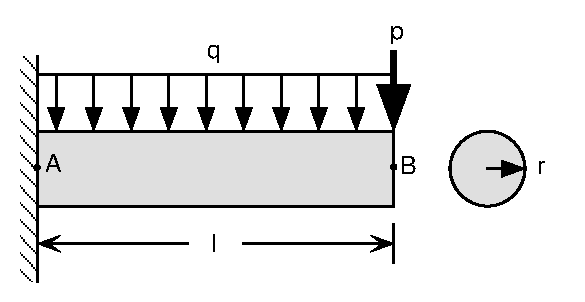
\includegraphics[clip=true]{beam.eps}
 \end{center}
\caption{Cantilever Beam}
\label{fig.beam}
\end{figure}
\begin{verbatim}
\begin{figure}[!htbp]
 \begin{center}
  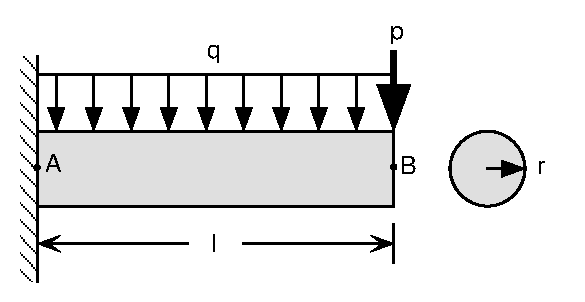
\includegraphics[clip=true]{beam.eps}
 \end{center}
\caption{Cantilever Beam}
\label{fig.beam}
\end{figure}
\end{verbatim}
Note the \enviro{figure} environment, which provides for captioning, and \enviro{center} environment for positioning the figure.

Figures can also be pasted in by hand if you leave room for them.
The following commands will leave a vertical space of 2.5 inches with a caption.
\begin{verbatim}
\begin{figure}
\vspace{2.5in}
\caption{Caption for Figure and for List of Figures - up to 300 chars}
\end{figure}
\end{verbatim}
%======================================================================
\section{Tables}
%======================================================================
Tables are easy to generate in \LaTeX .
Simple tables can be produced with the \enviro{tabbing} environment, as seen
in Section~\ref{ssec.fontfam}.
The source for that table is as follows:
\begin{verbatim}
\begin{tabbing}
mmmmm\=mmmmmmmmmmmmm\= \kill
\>\textbf{Command} \>\textbf{Description} \\
\>\cmmd{textrm} \>roman family \\
\>\cmmd{textsf} \>sans serif family \\
\>\cmmd{texttt} \>typewriter family \\
\>\cmmd{textbf} \>bold series \\
\>\cmmd{textmd} \>medium series \\
\>\cmmd{textit} \>italic shape \\
\>\cmmd{textsl} \>slanted shape \\
\>\cmmd{textup} \>upright shape (default)
\end{tabbing}
\end{verbatim}
Tabs are set with \cmmd{=}.
The \cmmd{kill} command cancels the line after the tabs are set. 
The \cmmd{>} moves to the next set tab stop.

The \enviro{table} and \enviro{tabular} environments can be used to produce captioned and bordered tables.
The following Table~\ref{tab.results} provides an example.
\begin{table}[!htbp]
\begin{center}
\begin{tabular}{|c||cc|cc|}
\hline
& \multicolumn{2}{c|}{ {\textbf CCP Rel. Indices} } 
& \multicolumn{2}{c|}{ {\textbf FORM Rel. Indices} } \\ 
\cline{2-5}
& $\beta_{MVFO}$ & $\beta_{MVMS}$ & $\beta_{FOSM}$ & $\beta_{FO}$ \\
\hline \hline
$\left\{ r^\star \, | \, \beta_1 \geq 3.719 \right\}$
& 1.347\dag & 1.348\dag & 1.325 & 1.175 \\
Rel. Error & +14.6\% & +14.7\% & +12.8\% & --- \\
%($\beta_2$) & (6.670) & (6.540) & (3.022) & (1.763) \\
\hline
$\left\{ r^\star \, | \, \beta_2 \geq 3.092 \right\}$
& 1.213 & 1.220 & 1.337\dag & 1.290\dag \\
Rel. Error & -6.0\% & -5.4\% & +3.6\% & --- \\
%($\beta_1$) & (3.222) & (3.251) & (3.755) & (4.742) \\
\hline
\end{tabular}
\begin{tabular}{l}
\footnotesize % smaller text in this environment only
\dag Active constraint when both are considered in the design 
optimization.
\end{tabular}
\end{center}
\caption{Minimum Beam Radius Using Four Reliability Indices}
\label{tab.results}
\end{table}
\begin{verbatim}
\begin{table}[!htbp]
\begin{center}
\begin{tabular}{|c||cc|cc|}
\hline
& \multicolumn{2}{c|}{ {\textbf CCP Rel. Indices} }
& \multicolumn{2}{c|}{ {\textbf FORM Rel. Indices} } \\
\cline{2-5}
& $\beta_{MVFO}$ & $\beta_{MVMS}$ & $\beta_{FOSM}$ & $\beta_{FO}$ \\
\hline \hline
$\left\{ r^\star \, | \, \beta_1 \geq 3.719 \right\}$
& 1.347\dag & 1.348\dag & 1.325 & 1.175 \\
Rel. Error & +14.6\% & +14.7\% & +12.8\% & --- \\
%($\beta_2$) & (6.670) & (6.540) & (3.022) & (1.763) \\
\hline
$\left\{ r^\star \, | \, \beta_2 \geq 3.092 \right\}$
& 1.213 & 1.220 & 1.337\dag & 1.290\dag \\
Rel. Error & -6.0\% & -5.4\% & +3.6\% & --- \\
%($\beta_1$) & (3.222) & (3.251) & (3.755) & (4.742) \\
\hline
\end{tabular}
\begin{tabular}{l}
\footnotesize % small text inside this environment only
\dag Active constraint when both are considered in the design 
optimization.
\end{tabular}
\end{center}
\caption{Minimum Beam Radius Using Four Reliability Indices}
\label{tab.results}
\end{table}
\end{verbatim}
Note that a second \enviro{tabular} environment was used to produce a footnote under the table.
A \enviro{minipage} environment around the table could also have been used.
%======================================================================
\section{Math Structures}
%======================================================================
\LaTeX\ uses an intuitive language for formatting mathematics.
Some examples of the main math environments will give the idea.
%----------------------------------------------------------------------
\subsection{In-Line Math}
%----------------------------------------------------------------------
In-line math may be inserted between \cmmd{(} and \cmmd{)}, or \$ and \$ (the latter form being preferred since it is not fragile).
For example,
\begin{verbatim}
\rv{A} is a random matrix of size $m \times n$ ($m < n$).
\end{verbatim}
produces ``\rv{A} is a random matrix of size $m \times n$ ($m < n$)''.
%----------------------------------------------------------------------
\subsection{Displayed Formulae}
%----------------------------------------------------------------------
Math may also be displayed (set apart from the text) with the \enviro{displaymath}, or between the short-cut commands \cmmd{[} and \cmmd{]}.
For example,
\begin{verbatim}
\begin{displaymath}
\beta \equiv \Phi^{-1}( \gamma )
\end{displaymath}
\end{verbatim}
produces
\begin{displaymath}
\beta \equiv \Phi^{-1}( \gamma )
\end{displaymath}
%----------------------------------------------------------------------
\subsection{Numbered Equations}
%----------------------------------------------------------------------
Numbered equations are produced inside the \enviro{equation} environment.
For example,
\begin{verbatim}
\begin{equation}
\label{eqn.gradbetaFO}
\nabla_D \beta_{FO} = \nabla_D \beta_{FOSM} =
\frac{ \nabla_{D} g_{i} (U^{\star} }{ \| \nabla_{U} g_{i} 
(U^{\star}) \| }
\end{equation}
\end{verbatim}
produces
\begin{equation}
\label{eqn.gradbetaFO}
\nabla_D \beta_{FO} = \nabla_D \beta_{FOSM} =
\frac{ \nabla_{D} g_{i} (U^{\star}) }{ \| \nabla_{U} g_{i} 
(U^{\star}) \| }
\end{equation}
%----------------------------------------------------------------------
\subsection{Equation Arrays}
%----------------------------------------------------------------------
The \enviro{eqnarray} produces equation arrays, which are structures for multi-line formulae.
Each line is given a number, unless this is suppressed with \cmmd{nonumber} command.
Numbering may be suppressed for the whole environment if the \enviro{eqnarray*} form of the environment command is used.
For example,
\begin{eqnarray}
  {\mathrm optimize} & \rv{C}^{T} X  \label{eqn.lpobjective} \\
  {\mathrm subject \: to} & \rv{A} X \leq  \rv{B} 
  \label{eqn.lpconstraints}
\end{eqnarray}
is produced by 
\begin{verbatim}
\begin{eqnarray}
  {\mathrm optimize} & \rv{C}^{T} X  \label{eqn.lpobjective} \\
  {\mathrm subject \: to} & \rv{A} X \leq  \rv{B} 
  \label{eqn.lpconstraints}
\end{eqnarray}
\end{verbatim}
Note that since each line is numbered, each may be given a label.
The \enviro{eqnarray} environment allows three columns, aligned on the \& symbols.
%----------------------------------------------------------------------
\subsection{Math Fonts}
\label{ssec.mathfonts}
%----------------------------------------------------------------------
Just as there are different type styles available in text mode, there are also math mode type styles, summarized below.
\begin{tabbing}
mmmmm\=mmmmmmmmmmmmm\= \kill
\>\textbf{Command} \>\textbf{Description} \\
\>\cmmd{mathrm} \>$\mathrm{roman}$ family\\
\>\cmmd{mathsf} \>$\mathsf{sans \: serif}$ family\\
\>\cmmd{mathtt} \>$\mathtt{typewriter}$ family\\
\>\cmmd{mathbf} \>$\mathbf{bold}$ series\\
\>\cmmd{mathit} \>$\mathit{italic}$ shape\\
\>\cmmd{mathcal} \>$\mathcal{CALIGRAPHIC}$ shape (upper case only)
\end{tabbing}
These commands only change the style of letters, numbers, and uppercase Greek letters, not other math symbols.
%======================================================================
\section{Appendices}
%======================================================================
Appendices may be included by simply adding an \cmmd{appendix} command in your master document.
All logical structures (chapters, sections, \etc) which appear below that point will then be ``numbered'' with letters.
%======================================================================
\section{Bibliography}
%======================================================================
A bibliography can be created two ways in \LaTeX , ``by hand'' or by using the \program{bibtex} program.
Once the bibliography items have been created by one of these methods, they are referred to in the \LaTeX\ source files with the \cmmd{cite} command. 
For example,
\begin{verbatim}
\LaTeX\ is a set of macros by Leslie Lamport \cite{lamport.book}.
\end{verbatim}
%----------------------------------------------------------------------
\subsection{``By-Hand'' Method}
%----------------------------------------------------------------------
In the ``End Material'' section of your master source file include your bibliography list, which you must format yourself. 
For example,
\begin{verbatim}
\begin{thebibliography}{9}
\bibitem{jungle.book} Jungle, George 
        {\em Watch Out for That Tree}
        Toronto: University of Toronto Press, 1986.
\bibitem{cliches.book} Smith, J.\ Henry.  
        {\em Cliches and Platitudes for Every Occasion}
        Ottawa: Political Press, 1996
\end{thebibliography}
\end{verbatim}
The second argument in the \cmmd{begin\{thebibliography\}\{9\}} is a number greater than the number of references to be formatted.  
The label parameter in the \cmmd{bibitem} command is used in the \cmmd{cite} command.
%----------------------------------------------------------------------
\subsection{Using BibTeX}
%----------------------------------------------------------------------
It is often easier to keep your bibliographic data together in bibliographic databases.
The \program{bibtex} program works with \LaTeX\ by gathering cited references from specified databases (text files with extension \exten{bib}, called \exten{BIB} files) and formatting the bibliography according to a desired style.
This method is much easier than doing the formatting ``by hand''.
If you create your own \exten{BIB} files, put them in the same directory as your \LaTeX\ source files, or set \program{latex}'s BIBINPUTS environment variable (under Unix) to the correct path.

The \program{bibtex} program is run after the \program{latex} program since it uses the \exten{AUX} files produced by \program{latex}.
The style and position of the bibliography in the final document is indicated by inserting the \cmmd{bibstyle} and \cmmd{bibliography} commands in the master \LaTeX\ source file.
The bibliography section by default does not appear in the Table of Contents. 
Adding it just requires manual editing of the file with extension \exten{TOC}, produced by \program{latex}, followed by a final run of \program{latex}.

The bibliography is formated according to the specified \cmmd{bibstyle} for each type of reference given: books, journals, collections, \etc .
The \texttt{bib} file used for this document is given below.
\begin{verbatim}
% Bibliography of key references for "LaTeX for Thesis 
% and Large Documents"
% For use with BibTeX

@book{goossens.book,
        author =	"Michel Goossens and Frank Mittelbach and 
        		 Alexander Samarin",
        title =		"The \LaTeX\ Companion",
        year = 		"1994",
        publisher =	"Addison-Wesley",
        address = 	"Reading, Massachusetts"
}

@book{knuth.book,
        author =        "Donald Knuth",
        title =         "The \TeX book",
        year =          "1986",
        publisher =     "Addison-Wesley",
        address =       "Reading, Massachusetts"
}

@book{lamport.book,
        author =        "Leslie Lamport",
        title =         "\LaTeX\ --- A Document Preparation System",
        edition =       "Second",
        year = 		"1994",
        publisher = 	"Addison-Wesley",
        address =       "Reading, Massachusetts"
}
\end{verbatim}
%======================================================================
\section{Glossary} 
%======================================================================
There is no specific \LaTeX\ command for creating a glossary.
However, one can easily be produced with the \enviro{description} environment, as shown in Appendix~\ref{chap.glossary}. 

The \program{makeindex} program can also be used to create a Glossary automatically, if terms are defined in specific places in your document.
%======================================================================
\section{Index}
%======================================================================
An index can be created two ways in \LaTeX , ``by hand'' or by using the \program{makeindex} program.
%----------------------------------------------------------------------
\subsection{``By-Hand'' Method}
%----------------------------------------------------------------------
In the ``End Material'' section of your master source file include your index with the \enviro{theindex} environment, then format it yourself.
For example,
\begin{verbatim}
\begin{theindex}
\item \LaTeX 3
   \subitem program, 4
      \subsubitem running, 5
\indexspace
\item \program{bibtex} 12
   \subitem running, 13
\end{theindex}
\end{verbatim}
%----------------------------------------------------------------------
\subsection{Using MakeIndex}
%----------------------------------------------------------------------
Use of the \program{makeindex} progam is recommended as a significant improvement over producing an index by hand.
If using \program{makeindex}, indexed items are
referred to in the \LaTeX\ source files with the \cmmd{index} command.
For example,
\begin{verbatim}
\LaTeX\index{\LaTeX} is a set of macros ...
\end{verbatim}
There are several other variations of the \cmmd{index} command which assist in formatting and ordering the index items.

To use \program{makeindex}, put a \verb=\usepackage{makeidx}= command in the preamble of your master source file.
If the command \cmmd{makeindex} also exists in the preamble of your master source file, \LaTeX\ will produce an \exten{IDX} file which is processed by \program{makeindex} to produce the final \exten{IND} file.
The \cmmd{printindex} command is placed in the master source document where you want the index to go in the end material.
Running \program{latex} again will place the index in the output \exten{DVI} file.
Note also that the index does not by default appear in the Table of Contents.
It must be added by hand, as was done for the Bibliography.
